\chapter{Matchings}
\lecture{6}{17 March.}{}
\begin{eg}
    \(n\) friends going for dinner. \(n\) bowls of beef noodle soup served. Each person has a subset of the bowls they would be happy with. Can we give one bowl to each person and making every one happy?  
\end{eg}
\begin{explanation}
    We can build a graph as follow: 
    \begin{figure}[H]
        \centering
        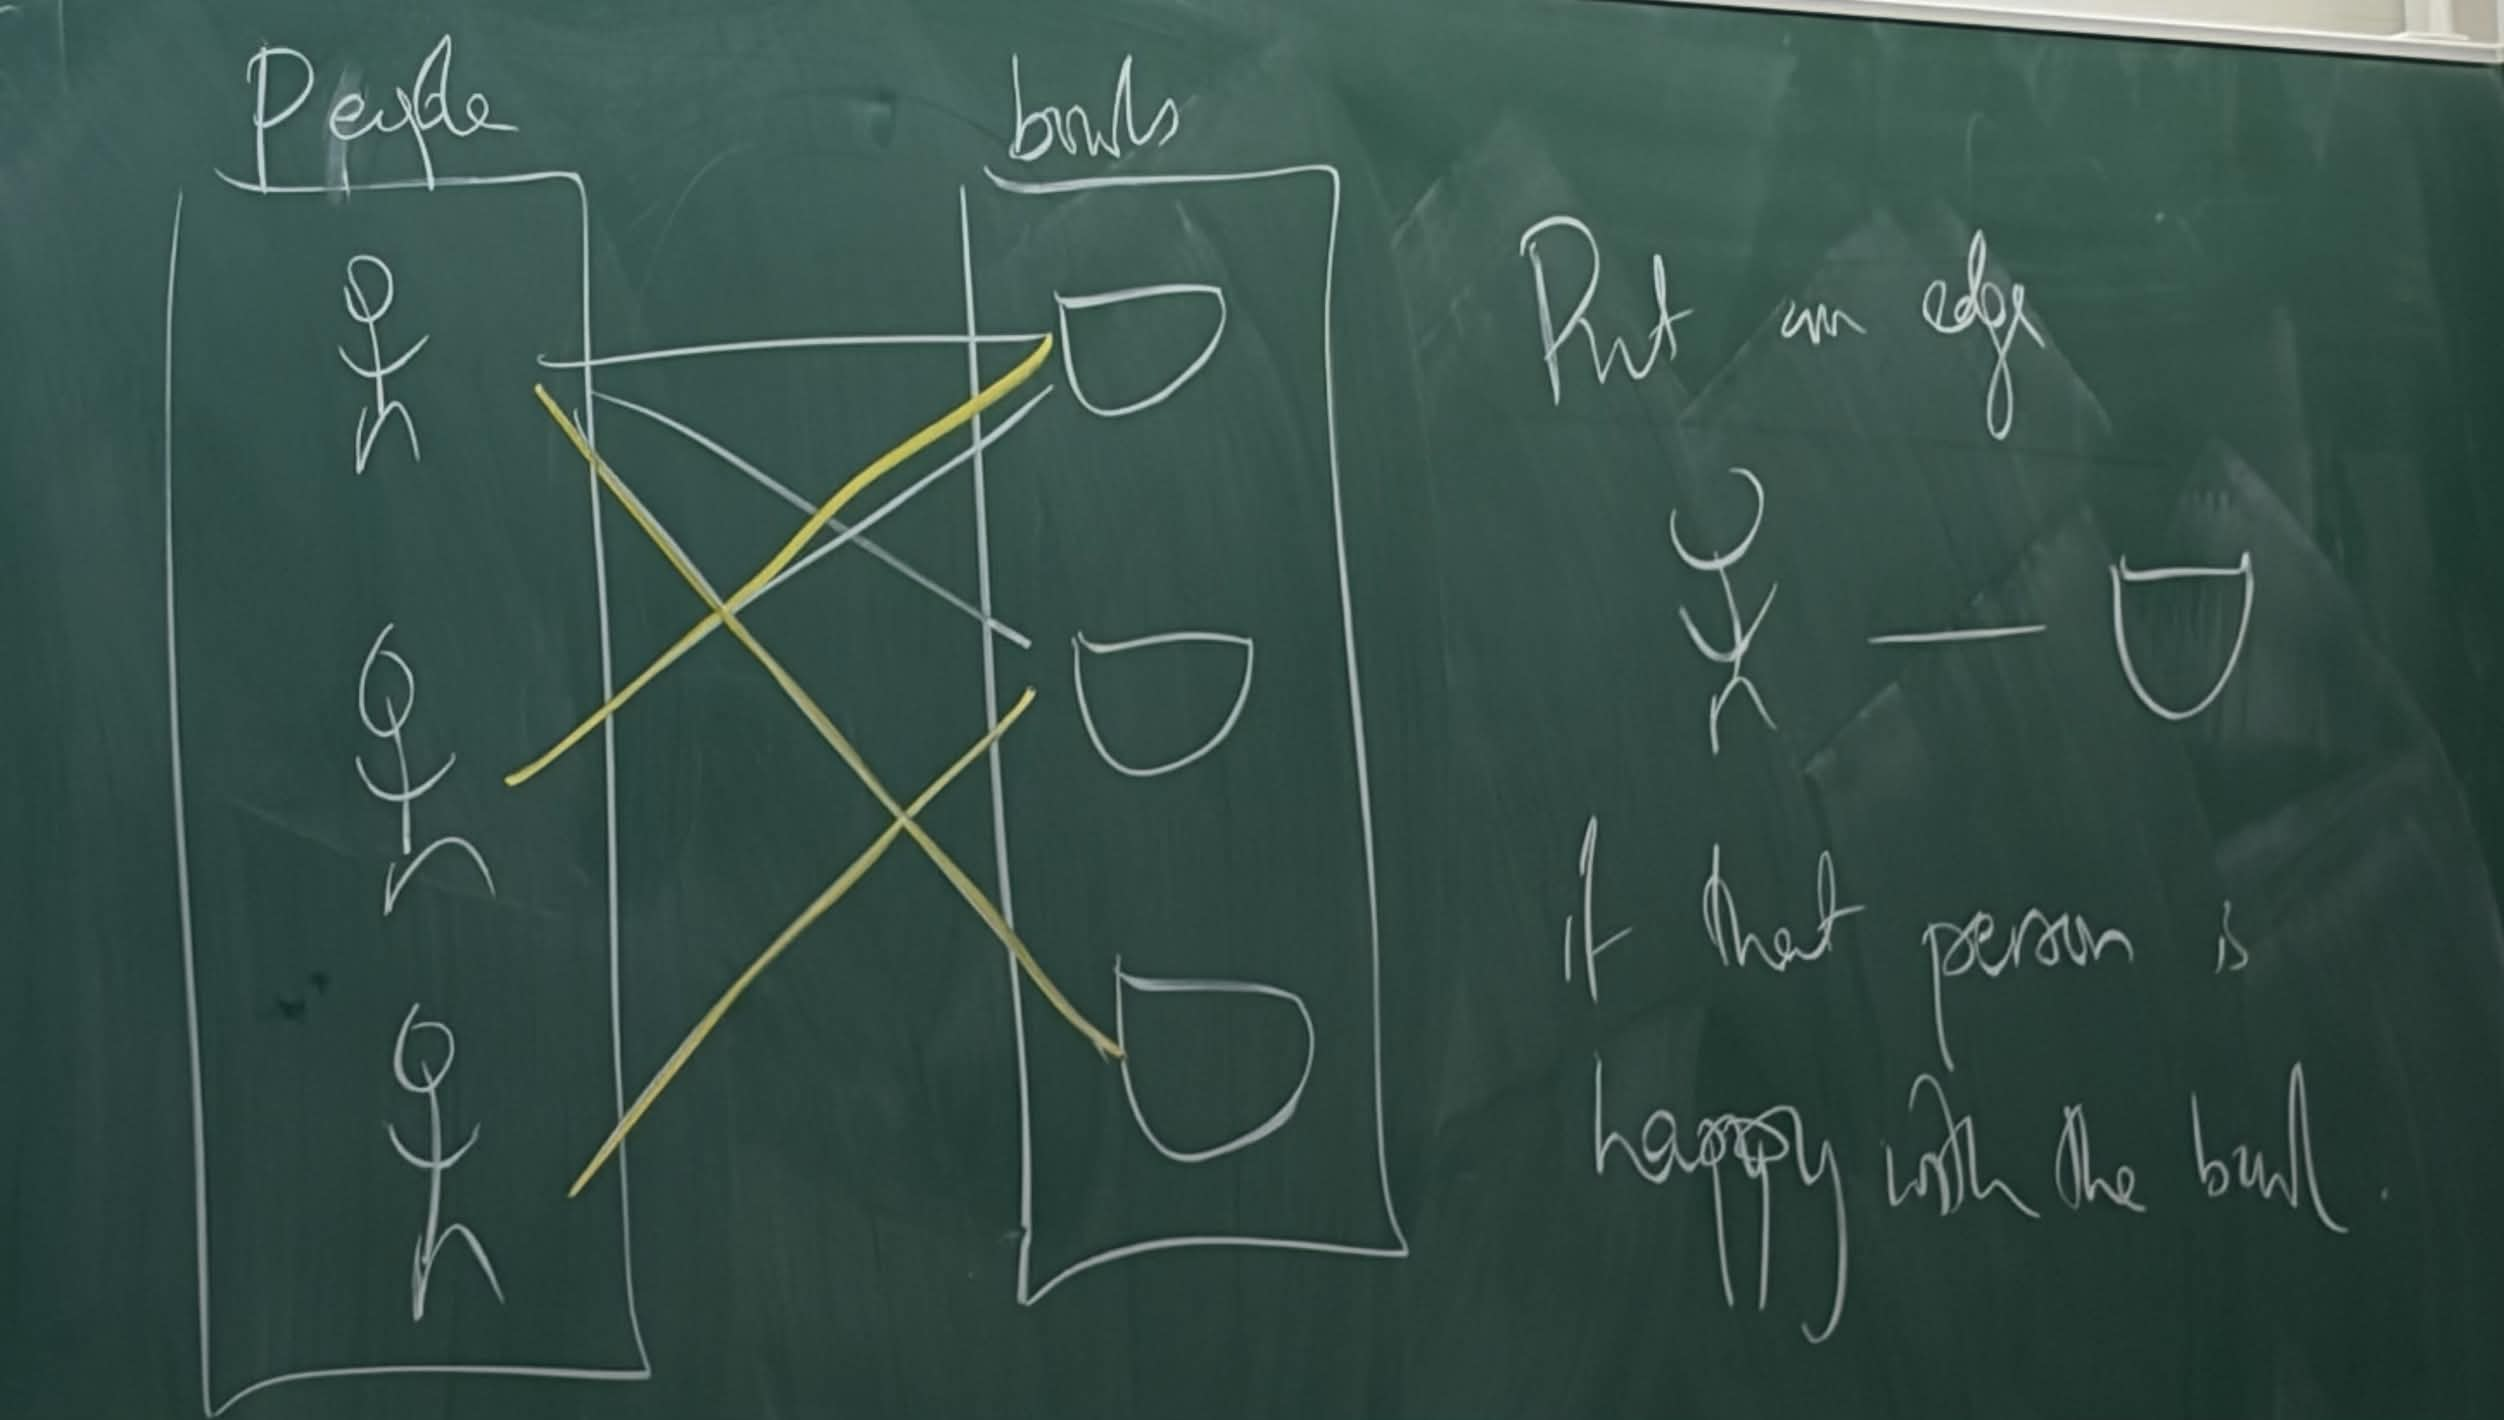
\includegraphics[width=0.6\textwidth]{./Figures/people_and_bowl.jpg}
    \end{figure}
\end{explanation}

\begin{definition}
    A graph \(G\) is bipartite if we can partition \(V(G) = X \cupdot Y\) s.t. for every \(e \in E(G)\),
    \[
        \vert e \cap X \vert = 1 = \vert e \cap Y \vert.
    \]   
\end{definition}

\begin{definition}
    A matching in a graph is a set of pairwise-disjoint edges. If a vertex is in an edge of the matching, it is called "saturated". If every vertex is saturated, the matching is perfect.
\end{definition}

\begin{observation}
    If there is some \(S \subseteq X\) with \(\vert N(S) \vert < \vert S \vert  \), then there is no matching saturating \(X\). 
\end{observation}
\begin{proof}
    If there is a matching saturating \(X\) and \(\exists S \subseteq X\) with \(\vert N(S) \vert < \vert S \vert  \), then each vertex in \(S\) would match with some vertex in \(N(S)\) in the matching saturating \(X\). Note that every vertex in \(S\) cannot match to same vertex. Hence, \(\vert N(S) \vert \ge \vert S \vert  \), which is a contradiction.    
\end{proof}

\begin{theorem}[Hall's Marriage Theorem]
    Let \(G = (X \cupdot Y, E)\) be a bipartite graph. If \(\vert N(S) \vert \ge \vert S \vert  \) for all \(S \subseteq X\), then \(G\) has a matching saturating \(X\).  
\end{theorem}

\begin{proof}
    We can do induction on \(\vert X \vert \). 
    \begin{itemize}
        \item Base case: \(\vert X \vert = 1 \). Let \(S = X\), and \(\vert N(X) \vert \ge \vert X \vert = 1\), then there exists \(y \in Y\) s.t. \(\left\{ x, y \right\} \in E \), so we can pick this edge to form a matching saturating \(X\). 
        \item Induction Step: \(\vert X \vert \ge 2 \). 
        \begin{itemize}
            \item Case 1: \(\forall \varnothing \neq S \subsetneq X\), \(\vert N(S) \vert > \vert S \vert  \). Let \(\left\{ x, y \right\} \) be an arbitrary edge, where \(x \in X\) and \(y \in Y\). Let \(G^{\prime} = (X^{\prime} \cup Y^{\prime} , E^{\prime})\) where \(X^{\prime} = X - \left\{ x \right\} \), \(Y^{\prime} = Y - \left\{ y \right\} \), and \(E^{\prime} = E\vert_{X^{\prime}  \times Y^{\prime} }\). We use induction to find a matching \(M^{\prime} \) in \(G^{\prime} \) saturating \(X^{\prime} \). Then, \(M = M^{\prime} \cup \left\{ x, y \right\} \) is a matching saturating \(X\). Note that we can use induction hypothesis since for \(S \subseteq X^{\prime} \), \(N_{G^{\prime} }(S) = N_G(S) \setminus \left\{ y \right\} \). Hence, 
            \[
                \vert N_{G^{\prime} }(S) \vert \ge \vert N_G(S) \vert - 1 \ge \vert S \vert,   
            \]
            and thus we can find \(M^{\prime} \). 
            \item Case 2: there exists some \(\varnothing \neq X_1 \subsetneq X\) with \(\vert N(X_1) \vert = \vert X_1 \vert \). Let \(N(X_1) = Y_1\). Let \(X_2 = X \setminus X_1\), and \(Y_2 = Y \setminus Y_1\), and \(G_1 = G[X_1 \cup Y_1]\). By induction, \(G_1\) has a matching \(M_1\) saturating \(X_1\) since for all \(S \subseteq X_1\), we have \(S \subseteq X\) and thus 
            \[
                \vert N_G(S) \vert \ge \vert S \vert,  
            \]
            and note that \(N_{G_1}(S) = N_G(S) \) since \(N_G(S) \subseteq N_G(X_1) = Y_1\).     If we can find a matching \(M_2\) in \(G_2 = G[X_2 \cup Y_2]\), then \(M = M_1 \cup M_2\) is a matching saturating \(X\). Let \(S \subseteq X_2\). Consider \(S^{\prime} = S \cup X_1\). By assumption, \(\vert N_G(S^{\prime} ) \vert \ge \vert S^{\prime}  \vert  \). Note that \(\vert S^{\prime} \vert = \vert S \vert + \vert X_1 \vert   \). Hence, 
            \[
                N_G(S^{\prime} ) = N_G(S \cup X_1) = Y_1 \cup \underbrace{N_{G_2}(S)}_{\subseteq Y_2}.
            \]
            Note that \(N_G(S^{\prime} ) = Y_1 \cup N_{G_2}(S)\) is a disjoint union since for \(N_G(S)\), it is either in \(Y_1\) or not, if not, then it is in \(N_{G_2}(S)\).   
            This shows
            \[
                \vert S \vert + \vert X_1 \vert = \vert S^{\prime}  \vert \le \vert N_G(S^{\prime} ) \vert = \vert Y_1 \vert + \vert N_{G_2}(S) \vert = \vert X_1 \vert + \vert N_{G_2}(S) \vert.        
            \]
            Hence, \(\vert N_{G_2}(S) \vert \ge \vert S \vert  \) for all \(S \subseteq X_2\). By induction, we can find a matching \(M_2\) in \(G_2\) saturating \(X_2\).    
        \end{itemize}
    \end{itemize} 
\end{proof}

\begin{corollary}
    If \(G\) is a \(d\)-regular bipartite graph, then \(G\) has a perfect matching.   
\end{corollary}

\begin{proof}
    Given any \(S \subseteq X\), 
    \[
        d \vert S \vert = \#\left\{ \text{edges between } S, N(S)  \right\}  \le d \vert N(S) \vert  
    \] 
    since for vertices in \(N(S)\), they may be adjacent to vertex not in \(S\), so by Hall's theorem, there is a matching saturating \(X\), which is a perfect matching since
    \[
        d \vert X \vert = \#\left\{ \text{edges between } X, Y  \right\} = d \vert Y \vert,   
    \] 
    and thus \(\vert X \vert = \vert Y \vert  \). 
\end{proof}

\begin{question}
    What are necessary and sufficient conditions to have a perfect matching in general (i.e. non-bipartite) graph?
\end{question}

For necessary condition:
\begin{itemize}
    \item \(n\) should be even. 
    \item every vertex should has positive degree. 
    \item every connected components should be even.  
    \item for any \(S \subseteq V(G)\), \(o(G - S) \le \vert S \vert \), where \(o(G - S)\) is the number of odd components in \(G - S\).   
\end{itemize}

\begin{remark}
    For the last argument, it is because \(G\) has a perfect matching, and for the odd components in \(G - S\), there must be edges between them and \(S\), i.e. some vertices in those odd componenets must match with the vertex in \(S\), and thus \(o(G - S) \le \vert S \vert \).
    
    \begin{figure}[H]
        \centering
        \incfig{oddComponent}
    \end{figure}
\end{remark}

\begin{theorem}[Tutte, 1947]
    If \(o(G - S) \le \vert S \vert \) for every \(S \subseteq V(G)\), then \(G\) has a perfect matching.   
\end{theorem}
\begin{proof}[proof (Lovasz, 1975)]
    Note that for \(S = \varnothing\), we have \(o(G) \le \vert 0 \vert \), so \(\vert V(G) \vert \) is even. If \(G\) is complete, then \(G\) obviously has a perfect matching. Now we consider the case that \(G\) is not complete. Suppose for contradiction. \(G\) is a counterexample on \(n\) vertices with the maximum number of edges.      
    \begin{claim}
        \(\forall \left\{ x, y \right\} \notin E(G) \), \(G^{\prime} = G + \left\{ x, y \right\} \) has a perfect matching.  
    \end{claim} 
    \begin{explanation}
        We have to show \(G^{\prime} \) satisfies Tutte's condition. If so, then since \(G\) was a longest counterexample, \(G^{\prime} \) cannot be a counterexample, so \(G^{\prime} \) has a perfect matching. 

        Note that we have \(o(G - S) \le \vert S \vert \) for all \(S \subseteq V(G)\). If \(\left\{ x, y \right\} \cap S \neq \varnothing \), then \(o(G^{\prime} - S) = o(G - S)\). If \(\left\{ x, y \right\} \) is contained in a component of \(G - S\), components don't change, so \(o(G^{\prime} - S) \le \vert S \vert \). If \(\left\{ x, y \right\} \) connects two components of \(G - S\), then no matter what happens, 
        \[
            o(G^{\prime} - S) \le o(G - S) \le \vert S \vert. 
        \]  
    \end{explanation} 

    \begin{remark}
        The perfect matching must pick \(\left\{ x, y \right\} \), otherwise we have a perfect matching in \(G\).  
    \end{remark}
    Let \(U = \left\{ v \in G: \deg(v) = n - 1 \right\} \). 
    \begin{itemize}
        \item Case 1: Every component of \(G - U\) is a clique(complete subgraph). Each even clique admits a perfect matching. Each odd clique has a matching with only one unsaturated vertex. By Tutte's condition, number of odd cliques \(\le \vert U \vert \), say there are \(k\) odd cliques. Thus, we can match the unsaturated vertices to different vertices in \(U\). Note that there will be even number of unused vertices in \(U\) since
        \[
            \vert V(G) \vert = \vert U \vert + \sum \text{size of components},    
        \]
        and since \(\vert V(G) \vert \) is even, we have 
        \[
            \vert U \vert \equiv k \mod{2}. 
        \]
        This shows \(\vert U \vert - k \) is even, i.e. after we match the unsaturated vertex in each odd component to \(U\), the number of unused verteices in \(U\) is even,  and thus we can match them arbitrarily.  
        \item Case 2: There is a non-clique component in \(G \setminus U\). We can find the following configuration:
        \begin{figure}[H]
            \centering
            \incfig{configuration}
        \end{figure}
        The reason is in \(G \setminus U\), there must be \(x, y, z\) which do not form a triangle, otherwise every component is a clique. On the other hand, \(y \notin U\), so there exists some \(w\) that is not adjacent to \(y\).     
        Let \(\textcolor{purple}{M_1}\) be a perfect matching in \(G + \left\{ w, y \right\} \) and let \(\textcolor{blue}{M_2}\) be a perfect matching in \(G + \left\{ x, z \right\} \). Let \(G^{\prime} = M_1 \cup M_2\). Then the components of \(G^{\prime} \) are either isolated edges (really in \(G\)) or even edges, alternating \(M_1\) and \(M_2\) edges. 
        \begin{figure}[H]
            \centering
            \incfig{m1mwtype}
        \end{figure}
        To build a matching \(M\) of \(G\), we can take all edges that are components in \(G^{\prime}\). Consider the cycle component \(C\) in \(G^{\prime} \). If the edges \(\left\{ y, w \right\} \) is not in \(C\), then take the \(M_1\) edges. If the edge \(\left\{ x, z \right\} \) is not in \(C\), then take the \(M_2\) edges. If both edges are in \(C\): If we delete \(y\) from this cycle, then there remains a path with an even number of edges and odd number of vertices. We can delete one of \(x\) or \(z\) s.t. the two remaining paths both have an even number of vertices. Note that we have \(\left\{ y, z \right\}, \left\{ y, x \right\}  \) these two edges, so we can take the edges incident to the deleted pair and since the remaining two subpaths are of even vertices, so we can take alternating edges on two subpaths to form a matching.                          
    \end{itemize}
\end{proof}